\documentclass[10pt]{article}
\usepackage[margin=0.85in]{geometry}
\usepackage{graphicx}
\usepackage{xcolor}
\usepackage{enumitem}
\usepackage[hidelinks]{hyperref}
\usepackage{titlesec}
\definecolor{navy}{RGB}{31,95,168}
\definecolor{darkred}{RGB}{176,58,46}
\titleformat{\section}{\large\bfseries\color{navy}}{}{0pt}{}
\titlespacing{\section}{0pt}{9pt}{4pt}
\setlist[itemize]{leftmargin=*, itemsep=1.5pt, topsep=2pt}
\setlength{\parskip}{4pt}
\setlength{\parindent}{0pt}
\graphicspath{{../figures/}}
\pagestyle{empty}

\begin{document}

{\LARGE\bfseries\color{navy} Why American Students' Test Scores Fell --- and What the Evidence Says}\\[2pt]
{\large Policy brief accompanying \emph{Why Did American Student Achievement Decline?} \hfill June 2026}

\vspace{2pt}\hrule\vspace{6pt}

\textbf{The bottom line:} American students have lost roughly a decade and a half of academic progress. The losses began around 2013 --- seven years \emph{before} COVID --- and are concentrated almost entirely among the lowest-performing students. After testing every major explanation against national, state, district, school-sector, and international data, the evidence points to two distinct problems: a pre-pandemic erosion most consistent with the saturation of adolescent life by smartphones and social media, and an unrecovered pandemic shock now sustained by chronic absenteeism. Fixing either one alone will not be enough.

\section{What happened}
\begin{itemize}
\item \textbf{Scores peaked around 2013 and have fallen ever since.} By 2024, 8th-grade math was back to its 2000 level and 8th- and 12th-grade reading were the lowest ever recorded. The average 8th grader has lost the equivalent of about a full grade level since 2013.
\item \textbf{This is a crisis of the struggling student, not the average one.} Before the pandemic, scores for the top 10\% of students were flat or \emph{rising}; scores for the bottom 10\% were collapsing (down 13 points in 13-year-olds' math from 2012 to 2020 --- before any school closed; left panel of the figure below). The gap between high and low performers is now the widest ever measured.
\end{itemize}

\begin{center}
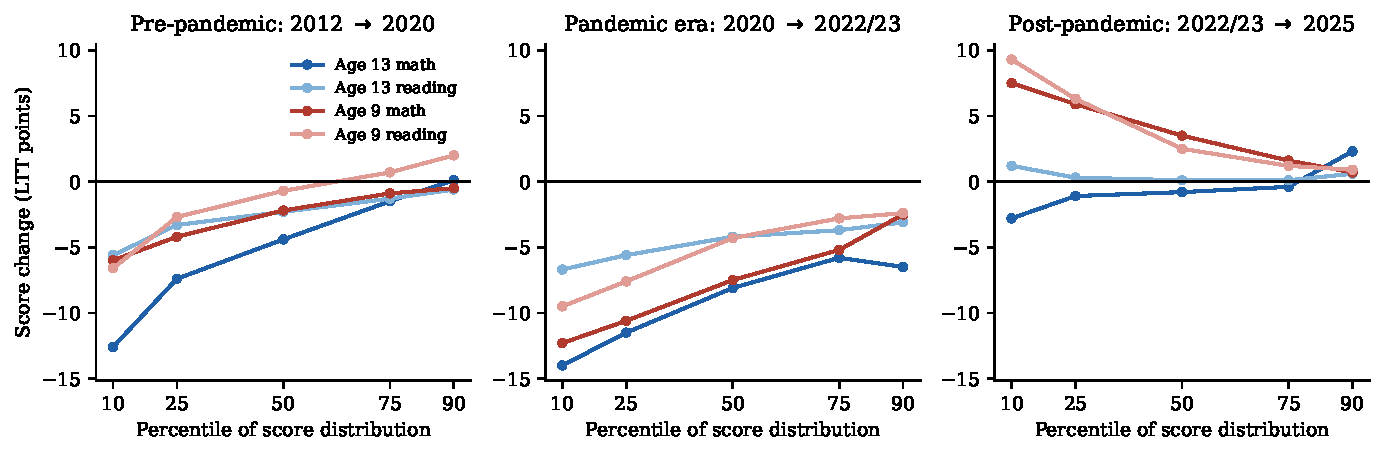
\includegraphics[width=.8\textwidth]{fig_ltt_percentiles.pdf}\\
{\footnotesize\textit{Score changes by student percentile (national long-term trend assessment, ages 9 and 13). Left: before the pandemic, losses were confined to lower-performing students while top students held steady. Right: the pandemic-era drop hit students at every level --- hardest at the bottom.}}
\end{center}

\begin{itemize}
\item \textbf{COVID made everything worse, and recovery has stalled.} The pandemic-era drop hit students at every level (right panel above), and four years later there has been essentially no rebound: reading is still falling, and the bottom of the distribution keeps sinking even as top students recover.
\item \textbf{It is not just a school problem --- or just an American one.} The same pattern appears in Catholic schools, in dozens of other wealthy countries, and --- strikingly --- among \emph{adults}: U.S. adult literacy fell 12 points from 2017 to 2023, with the same concentration at the bottom, across 19 OECD countries.
\end{itemize}

\section{What did \emph{not} cause the decline}
The analysis directly tested the most common explanations. Each failed:
\begin{itemize}
\item \textbf{Changing demographics?} No --- scores fell within every racial, ethnic, and income group; composition shifts explain at most 1--2 points.
\item \textbf{School funding cuts?} No --- spending recovered after 2013 while scores kept falling, and credible estimates of money's effect are far too small to explain the drop.
\item \textbf{Common Core?} No --- the four states that never adopted it declined just as much, or more.
\item \textbf{The end of No Child Left Behind accountability?} Largely no --- states released earlier from federal accountability fared no differently from states released later or never, in a test powered to detect half the effect accountability is credited with. (Accountability may still matter at the margins, especially in elementary grades.)
\item \textbf{Students just stopped trying on tests?} No --- self-reported test effort barely moved, behavioral indicators were stable, and the same decline shows up on state tests that carry real consequences and among adults.
\item \textbf{A measurement artifact?} No --- exclusion and participation rates were essentially unchanged throughout.
\end{itemize}

\section{What the evidence points to}
\textbf{Phase one (2013--2019): the smartphone era.} The decline began exactly when smartphones saturated teenage life (23\% of teens in 2011, 95\% by 2018). It struck adolescents specifically --- the same children who looked fine at age 9 fell behind by age 13 --- in public and private schools alike, in nearly every wealthy country, and among adults. Daily reading for fun among 13-year-olds halved. Heavy, poorly regulated device use is concentrated precisely among the lowest-performing students (and \emph{not} concentrated among low-income students). And when schools remove phones, rigorous studies in England, Norway, Spain, and Florida find achievement gains --- largest for exactly the struggling students who have driven the decline.

\textbf{Phase two (2020--present): disruption that became disengagement.} School closures caused the historic 2019--2022 drop --- that is settled science --- but the deeper problem is what followed: chronic absenteeism nearly doubled and remains roughly 50\% above pre-pandemic levels, and it now accounts for a quarter to two-fifths of the post-2019 decline. Students never fully came back.

\section{What policymakers can do}
\begin{itemize}
\item \textbf{Treat attendance as the front line of recovery.} No intervention works on students who are not there; absenteeism is the single largest identifiable drag on recovery.
\item \textbf{Take school phone restrictions seriously --- and bind them.} The causal evidence favors enforced, bell-to-bell restrictions (half-measures showed no effect in Sweden). About thirty states have now acted; the 2026 national assessment will deliver the decisive verdict, and this project has pre-registered that test.
\item \textbf{Target the bottom of the distribution.} Average-score goals miss the crisis. Mississippi's early-literacy reform --- intensive, monitored, early-grades instruction --- moved the state from 49th toward the national average and shows the floor can be raised by deliberate policy.
\item \textbf{Do not assume ``post-COVID recovery'' is the goal.} Returning to 2019 means returning to a downward trajectory. The pre-pandemic forces --- screens, disengagement, collapsing reading habits --- are still operating.
\end{itemize}

\vspace{4pt}\hrule\vspace{4pt}
{\footnotesize All findings are documented, with data and replication code, in the full 30-page report: national NAEP, Long-Term Trend, state and urban-district data pulled directly from federal sources; PISA, TIMSS, and PIAAC international data; and 600,000-student PISA microdata. Key sources include NCES/NAEP, OECD, the Education Recovery Scorecard, and peer-reviewed studies cited therein.}

\end{document}
